\documentclass[11pt]{report}
\usepackage[margin=2cm]{geometry}
\usepackage{graphicx}
\usepackage{float}
\usepackage{times}
\usepackage{url}
\usepackage[dvipsnames]{xcolor}
\usepackage{comment}

\newcommand{\et}{et al.~} 
\newcommand{\cd}{CO$_2$~}

\newcommand{\Gap}{\texorpdfstring{\hfill}{}}
\newcommand{\Rec}{\texorpdfstring{{\small\emph{\color{blue}{\fbox{High Leverage}}}}}{}}
\newcommand{\HighRisk}{\texorpdfstring{{\small\emph{\color{orange}{\fbox{Uncertain Impact}}}}}{}}
\newcommand{\Longterm}{\texorpdfstring{{\small\emph{\color{OliveGreen}{\fbox{Long-term}}}}}{}}

\begin{document}

\section{Buildings \& Cities\texorpdfstring{\hfill\textit{by Nikola Milojevic-Dupont and Lynn H.~Kaack}}{}}
\label{sec:buildings-cities}
Buildings offer some of the lowest-hanging fruit when it comes to reducing GHG emissions. While the energy consumed in buildings is responsible for a quarter of global energy-related emissions \cite{ipcc_global_2018}, a combination of easy-to-implement fixes and state-of-the-art strategies\footnote{The IPCC classifies mitigation actions in buildings into four categories: \textit{carbon efficiency} (switching to low-carbon fuels or to natural refrigerants); \textit{energy efficiency} (reducing energy waste through insulation, efficient appliances, better heating and ventilation, or other similar measures); \textit{system and infrastructure efficiency} (e.g.~passive house standards, urban planning, and district cooling and heating); and \textit{service demand reduction} (behavioral and lifestyle changes) \cite{lucon_buildings_2014}.} could reduce emissions for existing buildings by up to 90\% \cite{urge2013energy}. It is possible today for buildings to consume almost no energy \cite{OLSTHOORN20191382}.\footnote{There are even high-rise buildings, e.g. the Tower Raiffeisen-Holding N\"O-Vienna office, or large university buildings, e.g.~the Technical University also in Vienna, that achieve such performance.} Many of these energy efficiency measures actually result in overall cost savings \cite{STEPHENSON20106120} and simultaneously yield other benefits, such as cleaner air for occupants. This potential can be achieved while maintaining the services that buildings provide -- and even while extending them to more people, as climate change will necessitate. For example, with the changing climate, more people will need access to air conditioning in regions where deadly heat waves will become common \cite{mora2017twenty,mora2017global}. 


Two major challenges are heterogeneity and inertia. Buildings vary according to age, construction, usage, and ownership, so optimal strategies vary widely depending on the context. For instance, buildings with access to cheap, low-carbon electricity may have less need for expensive features such as intelligent light bulbs. Buildings also have very long lifespans; thus, it is necessary both to create new, energy-efficient buildings, and to retrofit old buildings to be as efficient as possible \cite{creutzig_urban_2016}. Urban planning and public policy can play a major role in reducing emissions by providing infrastructure, financial incentives, or energy standards for buildings.\footnote{For example, see the case of New York City, which mandated that building owners collectively reduce their emissions by 40\% by 2040: \url{https://www.nytimes.com/2019/04/17/nyregion/nyc-energy-laws.html}.}

Machine learning provides critical tools for supporting both building managers and  policy makers in their efforts to reduce GHG emissions (Fig.~\ref{fig:buildingsncities}). At the level of building management, ML can help select strategies that are tailored to individual buildings, and can also contribute to implementing those strategies via smart control systems (\S\ref{sec:indv}). At the level of urban planning, ML can be used to gather and make sense of data to inform policy makers (\S\ref{sec:distr}). Finally, we consider how ML can help cities as a whole to transition to low-carbon futures (\S\ref{sec:cities}).  

\begin{figure}
    \centering
    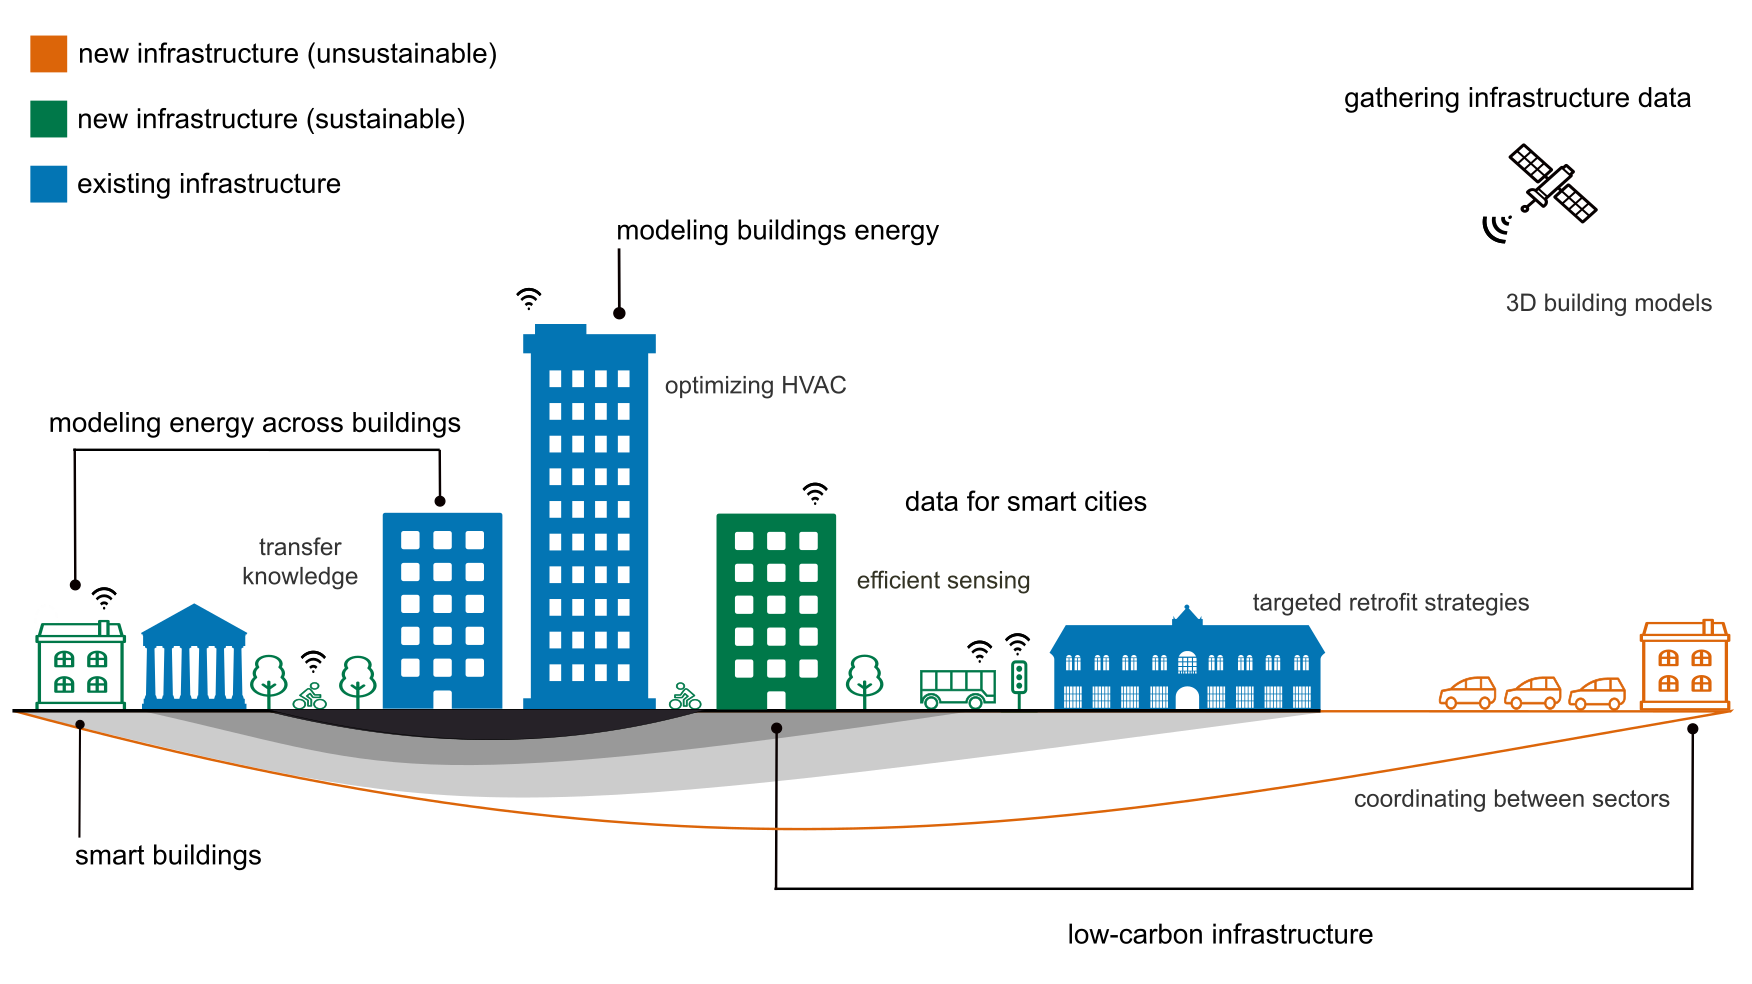
\includegraphics[width=\textwidth]{figures/building_n_cities.png}
    \caption{Selected strategies to mitigate GHG emissions from buildings and cities using machine learning.}
    \label{fig:buildingsncities}
\end{figure}

\subsection{Optimizing buildings}\label{sec:indv}
In designing new buildings and improving existing ones, there are numerous technologies that can reduce GHG emissions, often saving money in the process \cite{lucon_buildings_2014,urge2013energy,OLSTHOORN20191382,STEPHENSON20106120,Gershenfeld:2010aa}. ML can accelerate these strategies by (i) modeling data on energy consumption and (ii) optimizing energy use (in \emph{smart buildings}). 
 
\paragraph{Modeling building energy}\mbox{}\\\label{sec:use}An essential step towards energy efficiency is making sense of the increasing amounts of data produced by meters and home energy monitors (see for example \cite{sense}). This can take the form of energy demand forecasts for specific buildings, which are useful for power companies (\S\ref{sec:electricity-variable}) and in evaluating building design and operation strategies \cite{AMASYALI20181192}. Traditionally, energy demand forecasts are based on models of the physical structure of a building that are essentially massive thermodynamics computations. ML has the potential to speed up these computations greatly, either by ignoring physical knowledge of the building entirely \cite{kreider1995building,paterakis2017deep}, by incorporating it into the computation \cite{dong2016hybrid}, or by learning to approximate the physical model to reduce the need for expensive simulation (\emph{surrogate models}) \cite{VANGELDER2014245}. Learning how to transfer the knowledge gained from modeling one building to another can make it easier to render precise estimations of more buildings. For instance, Mocanu \et \cite{mocanu_unsupervised_2016} modeled building load profiles with reinforcement learning and deep belief networks using data on commercial and residential buildings; they then used approximate reinforcement learning and transfer learning to make predictions about new buildings, enabling the transfer of knowledge from commercial to residential buildings, and from gas- to power-heated buildings.

Within a single building, understanding which appliances drive energy use (\emph{energy disaggregation}) is crucial for targeting efficiency measures, and can motivate behavioral changes. Promising ML approaches to this problem include hidden Markov models \cite{kolter2012approximate}, sparse  coding  algorithms for structured prediction
\cite{kolter2010energy}, harmonic analysis that picks out the ``signatures'' of individual appliances \cite{Srinivasan2006neural}, and deep neural networks \cite{Kelly:2015:NND:2821650.2821672}.

To verify the success or failure of energy efficiency interventions, statistical ML offers methods for causal inference. For example, Burlig \et \cite{burlig2017machine} used Lasso regression on hourly electricity consumption data from schools in California to find that energy efficiency interventions fall short of the expected savings. Such problems could represent a useful application of deep learning methods for counterfactual prediction \cite{hartford2017deep}.

\paragraph{Smart buildings}\Gap\textbf{\Rec}\mbox{}\\\label{sec:bldgopt}Intelligent control systems in buildings can decrease the carbon footprint both by reducing the energy consumed and by providing means to integrate lower-carbon sources into the electricity mix \cite{Gershenfeld1086}. Specifically, ML can reduce energy usage by allowing devices and systems to adapt to usage patterns. Further, buildings can respond to signals from the electricity grid, providing flexibility to the grid operator and lowering costs to the consumer (\S\ref{sec:dispatchDR}). 

Many critical systems inside buildings can be made radically more efficient. While this is also true for small appliances such as refrigerators and lightbulbs, we use the example of heating and cooling (HVAC) systems, both because they are notoriously inefficient and because they account for more than half of the energy consumed in buildings \cite{lucon_buildings_2014}. There are several promising ways to enhance HVAC operating performance, each providing substantial opportunities for using ML: forecasting what temperatures are needed throughout the system, better control to achieve those temperatures, and fault detection. Forecasting temperatures, as with modeling energy use in buildings, has traditionally been performed using detailed physical models of the system involved; however, ML approaches such as deep belief networks can potentially increase accuracy with less computational expense \cite{afroz2018modeling,fu2018deep} (see also \S\ref{sec:demandresponse}). For control, Kazmi \et \cite{kazmi_gigawatt-hour_2018} used deep reinforcement learning to achieve a scalable 20\% reduction of energy while requiring only three sensors: air temperature, water temperature, and energy use (see also \S\ref{sec:demandresponse} for similarly substantial gains in datacenter cooling). Finally, ML can automate building diagnostics and maintenance through fault-detection. For example, the energy efficiency of cooling systems can degrade if refrigerant levels are low \cite{KIM20121805}; ML approaches are well-suited to detect faults in these systems. Wang \et \cite{wang_fault_2017} treated HVAC fault-detection as a one-class classification problem, using only temperature readings for their predictions. Deep autoencoders can be used to simplify information about machine operation so that deep neural networks can then more easily predict multiple kinds of faults \cite{jia2016deep}.

Many systems within buildings -- such as lights and heating -- can also adjust how they operate based on whether a building or room is occupied, thereby improving both occupant comfort and energy use \cite{park2019lightlearn}. ML can help these systems dynamically adapt to changes in occupancy patterns \cite{rashidi2009keeping}. Moreover, occupancy detection itself represents an opportunity for ML algorithms, ranging from decision trees \cite{d2015occupancy,zhao_occupant_2014} to deep neural networks \cite{zou2018towards} that take input from occupancy sensors \cite{d2015occupancy}, WiFi signals \cite{zou2018towards,zou2019unsupervised}, or appliance power consumption data \cite{zhao_occupant_2014}.

In \S\ref{sec:dispatchDR}, we discussed how using variable low-carbon energy can mean that the supply and price of electricity varies over time. Thus, energy flexibility in buildings is increasingly useful to schedule consumption when supply is high \cite{riekstin2018time}.  For this, automated demand-side response \cite{hu2013hardware} can respond to electricity prices, smart meter signals, or learned user preferences \cite{JIN20171583}. Edge computing can be used to process data from distributed sensors and other \emph{Internet of Things} devices, and deep reinforcement learning can then use this data to efficiently schedule energy use \cite{liu2019intelligent}.

While smart building technologies have the capability to significantly increase efficiency, we should note that there are potential drawbacks \cite{hittinger2019internet}. First, smart building devices and connection networks, like wireless sensor networks, consume energy themselves; however, deep neural networks can be used to monitor and optimize their operations \cite{ateeq2019multi}.  Second, rebound effects are likely to happen in certain cases \cite{azevedo2014consumer}, leading to additional building energy consumption typically ranging between 10 and 20\% \cite{rau2018cross}. If control systems optimize for costs, interventions do not necessarily translate into energy efficiency measures or GHG reductions. Therefore, public policies are needed to mandate, support and complement the actions of individual building managers \cite{lucon_buildings_2014}.
Another concern in the case of widespread adoption of smart meters is the impact on mineral use and embodied energy use arising from their production \cite{sias2017characterization}. 
Finally, smart home applications present security and privacy risks \cite{couldry2019data} that require adequate regulation.

\subsection{Urban planning}\label{sec:distr}
For many impactful mitigation strategies -- such as district heating and cooling, neighborhood planning, and large-scale retrofitting of existing buildings -- coordination at the district and city level is essential. Policy makers use instruments such as building codes, retrofitting subsidies, investments in public utilities, and public-private partnerships in order to reduce GHG emissions without compromising equity.  
Where energy-use data on individual buildings exist, ML can be used to derive higher-level patterns. However, many regions of the world have almost no energy consumption data, which can make it difficult to design targeted mitigation strategies. ML is uniquely capable of predicting energy consumption and GHG mitigation potential at scale from other types of available data. 

\paragraph{Modeling energy use across buildings}\label{sec:bldg3d}\mbox{}\\
\emph{Urban Building Energy Models} provide simplified information on the energy use of all buildings across a city. These are different from individual-building models, which model energy use of only specific buildings, but with finer details and temporal granularity (\S\ref{sec:indv}). While UBEMs have yet to be adopted at scale, they are expected to become fundamental for enabling localized action by city planners \cite{reinhart_urban_2016}.\footnote{The startup nam.R is developing a database of all school buildings in France to help inform retrofitting decisions, harmonizing vast amounts of open and proprietary data with ML \cite{namr}.}  UBEMs can for example be used for planning and operating \emph{district heating and cooling}, where a central plant supplies many households in a district. In turn, district heating and cooling reduces HVAC energy consumption and can provide flexible load \cite{VANDERMEULEN2018103}, but it needs large amounts of data at the district level for implementation and operation. 


UBEMs include features such as the location, geometries, and various other attributes of interest like building footprint, usage, material, roof type, immediate surroundings etc. ML can be used to held predict energy consumption from such features. For example, Kolter and Ferreira used Gaussian process regression to predict energy use from features such as property class or the presence of central AC \cite{kolter_large-scale_2011}. Based on energy data disclosed by residents of New York City, Kontokosta and colleagues used various ML methods to predict the energy use of the city's 1.1 million buildings \cite{kontokosta2017data}, analyzed the effect of energy disclosure on the demand \cite{papadopoulos2018pattern}, and developed a system for ranking buildings based on energy efficiency \cite{PAPADOPOULOS2019244}. Zhang \et \cite{ZHANG2018162} matched residential energy consumption survey data with public use microdata samples to estimate residential energy consumption at the neighborhood level. Using five commonly accessible features of buildings and climate, Robinson et al.~predict commercial building energy use across large American cities \cite{robinson2017machine}.

Beyond energy prediction, buildings' features can be used by ML algorithms to pinpoint which buildings have the highest retrofit potential. Simple building characteristics and surrounding environmental factors -- both potentially available at scale -- can be used \cite{khayatian2017building, bocher2018geoprocessing}.

There have also been attempts to upscale individual-building energy models to the district scale. Using deep neural networks for hybrid ML-physical modelling, Nutkiewicz \et provided precise energy demand forecasts that account for inter-building energy dynamics and urban microclimate factors for all buildings on a campus \cite{nutkiewicz2018data}.


\paragraph{Gathering infrastructure data}\Gap\textbf{\Rec}\mbox{}\\%\HighImpact
\label{sec:bldginfrastructure}Specifics about building infrastructure can often be predicted using ML techniques.  
Remote sensing is key to inferring infrastructure data \cite{esch2017breaking,microsoftbuildings,yu2018deepsolar,LU2014134,Henn2012,blaha2016large} as satellite data\footnote{See \cite{zhu2017deep} for a review of different sources of data and deep learning methods for processing them.} present a source of information that is globally available and largely consistent worldwide. For example, using remote sensing data, Gei\ss \ \et \cite{Gei__2011} clustered buildings into types to assess the potential of district heat in a German town. 

The resolution of infrastructure data ranges from coarse localization of all buildings at the global scale \cite{esch2017breaking}, to precise 3D reconstruction of a neighborhood \cite{blaha2016large}. It is possible to produce a global map of human settlement footprints at meter-level resolution from satellite radar images \cite{esch2017breaking}. For this, Esch \et used highly automated learners, which make classification at such scale possible by retraining locally. Segmentation of high-resolution satellite images can now generate exact building footprints at a national scale \cite{microsoftbuildings}. Energy-relevant building attributes, such as the presence of photovoltaic panels, can also be retrieved from these images \cite{yu2018deepsolar} (see \S\ref{sec:electricity-variable}). 
To generate 3D models, LiDAR data is often used to retrieve heights or classify buildings at city scale \cite{LU2014134,Henn2012}, but its collection is expensive. 
Recent research showed that heights can be predicted even without such elevation data, as demonstrated by \cite{BILJECKI20171}, who predicted these from real estate records and census data. 
Studies, which for now are small scale, aim for complete 3D reconstruction with class labels for different components of buildings \cite{blaha2016large}. 

\subsection{The future of cities}\label{sec:cities}
Since most of the resources of the world are ultimately channeled into cities, municipal governments have a unique opportunity to mitigate climate change. City governments regulate (and sometimes operate) transportation, buildings, and economic activity. They handle such diverse issues as energy, water, waste, crime, health, and noise. Recently, data and ML have become more common for improving efficiency in such areas, giving rise to the notion of \emph{smart city}. While the phrase \emph{smart city} encompasses a wide array of technologies \cite{neirotti2014current}, here we discuss only applications that are relevant to reducing GHG emissions.

\paragraph{Data for smart cities}\Gap\Rec\mbox{}\\
\label{sec:data_pol}Increasingly, important aspects of city life come with digital information that can make the city function in a more coordinated way. Habibzadeh \et \cite{8291118} differentiate between \emph{hard-sensing}, i.e., fixed-location-dedicated sensors like traffic cameras, and \emph{soft-sensing}, for example from mobile devices. Hard sensing is the primary data collection paradigm in many smart city applications, as it is adapted to precisely meet the application requirements. However, there is a growing volume of data coming from soft sensing, due to the widespread adoption of personal devices like smartphones that can provide movement data and geotagged pictures.\footnote{Note that management of any such private data, even if they are anonymized, poses challenges \cite{creutzig_leveraging_2019}.} Urban computing \cite{urban-computing} is an emerging field looking at data analytics in urban spaces, and aiming to yield insights for data-driven policies. For example, clustering anonymized credit card payments makes it possible to model different communities and lifestyles -- of which the sustainability can be assessed \cite{di2018sequences}. Jiang \et provides a review of urban computing from mobile phone traces \cite{jiang2013review}.\footnote{See \url{https://www.microsoft.com/en-us/research/project/urban-computing/} for more applications of urban computing.} Relevant information on the urban space can also be learned from social media activity, e.g.~on Twitter, as reviewed in \cite{ilieva2018social, ruths2014social}.
There are, however, numerous challenges in making sense of this wealth of data (see \cite{mosannenzadeh2017identifying}), and privacy considerations are of paramount importance when collecting or working with many of these data sources.

First, cities need to obtain relevant data on activities that directly or indirectly consume energy. Data are often proprietary. To obtain these data, the city of Los Angeles now requires all \emph{mobility as a service} providers, i.e.~vehicle-sharing companies, to use an open-source API. Data on location, use, and condition of all those vehicles, which can be useful in guiding regulation, are thus transmitted to the city \cite{cityLAgit}. ML can also distill information on urban issues related to climate change through web-scraping and text-mining, e.g.~\cite{doi:10.1177/0361198119838982}. As discussed above (\S\ref{sec:distr}), ML can also be used to infer infrastructure data.

Second, smart city applications must transmit high volumes of data in real-time. ML is key to preprocessing large
amounts of data in large sensor networks, allowing only what is relevant to be transmitted, instead of all the raw
data that is being collected \cite{li2016geospatial, valerio2016hypothesis, ravi2017deep}. Similar techniques also help to reduce the amount of energy consumed during
transmission itself \cite{muhammad2019intelligent}.

Third, urban policy-making based on intelligent infrastructure faces major challenges with data management \cite{Giest_2017}.
Smart cities require the integration of multiple large and heterogeneous sources of data, for which ML can be a valuable tool, which includes data matching \cite{bordes2014semantic,doan2004ontology}, data fusion \cite{methodologies-for-cross-domain}, and ensemble learning \cite{krawczyk2017ensemble}.


\paragraph{Low-emissions infrastructure}\Gap\mbox{}\\\label{sec:smart_cities}When smart city projects are properly integrated into urban planning, they can make cities more sustainable and foster low-carbon lifestyles (see \cite{wu2016big,o2019smart,muhammad2019intelligent} for extensive reviews on this topic). Different types of infrastructure interact, meaning that planning strategies should be coordinated to achieve mitigation goals. For instance, urban sprawl influences the energy use from transport, as wider cities tend to be more car-oriented \cite{ewing_does_2017,creutzig_global_2015,ding2018applying}. ML-based analysis has shown that the development of efficient public transportation is dependent on both the extent of urban sprawl and the local development around transportation hubs \cite{silva2018scenario,monajem2015evaluation}. 

Cities can reduce GHG emissions by coordinating between infrastructure sectors and better adapting services to the needs of the inhabitants. ML and AI can help, for example, to coordinate district heating and cooling networks, solar power generation, and charging stations for electric vehicles and bikes \cite{o2019smart}, and can improve public lighting systems by regulating light intensity based on historical patterns of foot traffic \cite{de2016intelligent}. Due to inherent variability in energy demand and supply, there is a need for uncertainty estimation, e.g.~using Markov chain Monte Carlo methods or Gaussian processes \cite{o2019smart}.


Currently, most smart city projects for urban climate change mitigation are implemented in wealthier regions such as the United States, China, and the EU.\footnote{See for example the European Union H2020 smart cities project  \url{https://ec.europa.eu/inea/en/horizon-2020/smart-cities-communities}.} 
The literature on city-scale mitigation strategies is also strongly biased towards the Global North \cite{lamb2019learning}, while key mitigation challenges are expected to arise from the Global South \cite{nagendra2018urban}. Infrastructure models described in \S\ref{sec:distr} could be used to plan low-carbon neighborhoods without relying on advanced smart city technologies. To transfer strategies across cities, it is possible to cluster similar cities based on climate-relevant dimensions  \cite{han_1_nodate,louf_typology_2014}. Creutzig \et \cite{creutzig_global_2015} related the energy use of 300 cities worldwide to historical structural factors such as fuel taxes (which have a strong impact on urban sprawl).  Other relevant applications include groupings of transportation systems \cite{han_1_nodate} using a latent class choice model, or of street networks \cite{louf_typology_2014} to identify common patterns in urban development using hierarchical clustering.

\subsection{Discussion}
We have shown many different ways that ML can help to reduce GHG emissions from buildings and cities. A central challenge in this sector is the availability of high-quality data for training the algorithms, which rarely go beyond main cities or represent the full spectrum of building types. Techniques for obtaining these data, however, can themselves be an important application for ML (e.g.~via computer vision algorithms to parse satellite imagery). Realizing the potential of data-driven urban infrastructure can advance mitigation goals while improving the well-being of citizens \cite{urge2013energy,bai2018six,creutzig_urban_2016}.

% \bibliographystyle{unsrt}
% \bibliography{references}

\end{document}
